%!TEX TS-program = xelatex
%!TEX encoding = UTF-8 Unicode
% Awesome CV LaTeX Template for CV/Resume
%
% This template has been downloaded from:
% https://github.com/posquit0/Awesome-CV
%
% Author:
% Claud D. Park <posquit0.bj@gmail.com>
% http://www.posquit0.com
%
%
% Adapted to be an Rmarkdown template by Mitchell O'Hara-Wild
% 23 November 2018
%
% Template license:
% CC BY-SA 4.0 (https://creativecommons.org/licenses/by-sa/4.0/)
%
%-------------------------------------------------------------------------------
% CONFIGURATIONS
%-------------------------------------------------------------------------------
% A4 paper size by default, use 'letterpaper' for US letter
\documentclass[11pt,a4paper,]{awesome-cv}

% Configure page margins with geometry
\usepackage{geometry}
\geometry{left=1.4cm, top=.8cm, right=1.4cm, bottom=1.8cm, footskip=.5cm}


% Specify the location of the included fonts
\fontdir[fonts/]

% Color for highlights
% Awesome Colors: awesome-emerald, awesome-skyblue, awesome-red, awesome-pink, awesome-orange
%                 awesome-nephritis, awesome-concrete, awesome-darknight

\colorlet{awesome}{awesome-red}

% Colors for text
% Uncomment if you would like to specify your own color
% \definecolor{darktext}{HTML}{414141}
% \definecolor{text}{HTML}{333333}
% \definecolor{graytext}{HTML}{5D5D5D}
% \definecolor{lighttext}{HTML}{999999}

% Set false if you don't want to highlight section with awesome color
\setbool{acvSectionColorHighlight}{true}

% If you would like to change the social information separator from a pipe (|) to something else
\renewcommand{\acvHeaderSocialSep}{\quad\textbar\quad}

\def\endfirstpage{\newpage}

%-------------------------------------------------------------------------------
%	PERSONAL INFORMATION
%	Comment any of the lines below if they are not required
%-------------------------------------------------------------------------------
% Available options: circle|rectangle,edge/noedge,left/right

\photo{Foto\_cv.jpg}
\name{Juan Manuel}{Díaz López}

\position{Licenciado en Psicología con 6 años de experiencia en
investigación dentro del área educativa}
\address{México, CDMX}

\mobile{5533324614}
\email{\href{mailto:juan_dm@comunidad.unam.mx}{\nolinkurl{juan\_dm@comunidad.unam.mx}}}
\github{Juan9711}
\linkedin{\url{https://www.linkedin.com/in/juan-manuel-díaz-lópez-5b510b262/}}

% \gitlab{gitlab-id}
% \stackoverflow{SO-id}{SO-name}
% \skype{skype-id}
% \reddit{reddit-id}


\usepackage{booktabs}

\providecommand{\tightlist}{%
	\setlength{\itemsep}{0pt}\setlength{\parskip}{0pt}}

%------------------------------------------------------------------------------



% Pandoc CSL macros
\newlength{\cslhangindent}
\setlength{\cslhangindent}{1.5em}
\newlength{\csllabelwidth}
\setlength{\csllabelwidth}{2em}
\newenvironment{CSLReferences}[3] % #1 hanging-ident, #2 entry spacing
 {% don't indent paragraphs
  \setlength{\parindent}{0pt}
  % turn on hanging indent if param 1 is 1
  \ifodd #1 \everypar{\setlength{\hangindent}{\cslhangindent}}\ignorespaces\fi
  % set entry spacing
  \ifnum #2 > 0
  \setlength{\parskip}{#2\baselineskip}
  \fi
 }%
 {}
\usepackage{calc}
\newcommand{\CSLBlock}[1]{#1\hfill\break}
\newcommand{\CSLLeftMargin}[1]{\parbox[t]{\csllabelwidth}{\honortitlestyle{#1}}}
\newcommand{\CSLRightInline}[1]{\parbox[t]{\linewidth - \csllabelwidth}{\honordatestyle{#1}}}
\newcommand{\CSLIndent}[1]{\hspace{\cslhangindent}#1}

\begin{document}

% Print the header with above personal informations
% Give optional argument to change alignment(C: center, L: left, R: right)
\makecvheader

% Print the footer with 3 arguments(<left>, <center>, <right>)
% Leave any of these blank if they are not needed
% 2019-02-14 Chris Umphlett - add flexibility to the document name in footer, rather than have it be static Curriculum Vitae


%-------------------------------------------------------------------------------
%	CV/RESUME CONTENT
%	Each section is imported separately, open each file in turn to modify content
%------------------------------------------------------------------------------



\hypertarget{educaciuxf3n}{%
\section{Educación}\label{educaciuxf3n}}

\begin{cventries}
    \cventry{Licenciatura en Psicología}{Facultad de Psicología, UNAM}{Ciudad de México, México}{Titulado el 18 de noviembre del 2022}{\begin{cvitems}
\item Proyecto de titulación - ``Relación entre el desempeño en tareas de discriminación numérica, temporal y espacial en diferentes grupos de edad''
\end{cvitems}}
\end{cventries}

\hypertarget{experiencia-laboral}{%
\section{Experiencia laboral}\label{experiencia-laboral}}

\begin{cventries}
    \cventry{Prestador del servicio social}{UNAM, Laboratorio de estudios sobre desarrollo numérico}{Ciudad de México, México}{2017 - 2019}{\begin{cvitems}
\item Programación de tareas de evaluación para estudiantes de educación básica, investigación aplicada, análisis y reporte de datos, elaboración de marcos conceptuales, redacción de reportes de investigación, gestión de protocolos de investigación y manejo de grupos
\end{cvitems}}
    \cventry{Supervisor}{UNAM, Programa de iniciación tempra a la investigación (PiTIP)}{Ciudad de México, México}{2017-2022}{\begin{cvitems}
\item Manejo de grupos
\end{cvitems}}
    \cventry{Prestador de prácticas profesionales}{UNAM, Proyecto PAPIME  “Retos de la permanencia y el abandono escolar“}{Ciudad de México, México}{2018-2020}{\begin{cvitems}
\item Análisis y reporte de datos, elaboración de marcos conceptuales y búsqueda de información en bases especializadas
\end{cvitems}}
    \cventry{Asistente de proyecto}{Departamento de Matemática Educativa del Cinvestav}{Ciudad de México, México}{2020 - 2021}{\begin{cvitems}
\item Análisis y reporte de datos, elaboración de marcos conceptuales y búsqueda de información en bases especializadas
\end{cvitems}}
    \cventry{Coordinador de desarrollo de pruebas}{Computational Psychometrics Lab, convenio de colaboración UNAM-USICAMM}{Ciudad de México, México}{2021}{\begin{cvitems}
\item Generación y corrección de reactivos para evaluación a gran escala, elaboración de marcos conceptuales, búsqueda de información en bases especializadas y análisis/reporte de datos
\end{cvitems}}
    \cventry{Coordinador de desarrollo de reactivos}{Innova Schools}{Ciudad de México, México}{2021 - 2022}{\begin{cvitems}
\item Generación y redacción de reactivos para evaluaciones en educación básica en las áreas de comunicación, matemáticas y ciencias
\end{cvitems}}
\end{cventries}

\hypertarget{formaciuxf3n-complementaria}{%
\section{Formación complementaria}\label{formaciuxf3n-complementaria}}

\begin{cventries}
    \cventry{Curso - ``Búsqueda de información y biblioteca digital''}{UNAM, Facultad de Psicología}{Ciudad de México, México}{2015}{}\vspace{-4.0mm}
    \cventry{Curso - “Introducción a la programación y análisis estadístico con el lenguaje R”}{UNAM, Facultad de Psicología}{Ciudad de México, México}{2019}{}\vspace{-4.0mm}
    \cventry{Curso - ``Modelos Psicométricos - Tópicos selectos''}{UNAM, Facultad de Psicología}{Ciudad de México, México}{2019}{}\vspace{-4.0mm}
    \cventry{Curso - ``Aprende a diseñar reactivos de opción múltiple para exámenes''}{UNAM, Facultad de Psicología}{Ciudad de México, México}{2019}{}\vspace{-4.0mm}
    \cventry{Curso - ``Teoría de la validez contemporánea: Aplicaciones en ciencias sociales y de la salud''}{UNAM, Facultad de Psicología}{Ciudad de México, México}{2022}{}\vspace{-4.0mm}
\end{cventries}

\hypertarget{ponencias}{%
\section{Ponencias}\label{ponencias}}

\begin{cventries}
    \cventry{}{Ponencia - ``Caracterización del vínculo afectivo de amigovios''}{Asociación Mexicana de Psicología social}{2016}{}\vspace{-4.0mm}
    \cventry{}{Curso - ``Ciencia de datos con R: lo que no puedes hacer con SPSS''}{UNAM, Facultad de Psicología}{2019}{}\vspace{-4.0mm}
    \cventry{https://repository.ucatolica.edu.co/server/api/core/bitstreams/997221e5-af67-42b4-adea-9d67a6c2cd9f/content}{Ponencia - ``Estimación de la probabilidad de rezago en las asignaturas del plan de estudios de Psicología en la UNAM: Modelo de Rash''}{Universidad Católica De Colombia, VII Simposio Internacional de Psicología}{2021}{}\vspace{-4.0mm}
    \cventry{}{Curso - “Medición psicométrica contemporánea en Psicología: Aplicaciones en el campo educativo, organizacional y de la salud”}{UNAM, Facultad de Psicología}{2022}{}\vspace{-4.0mm}
\end{cventries}

\newpage

\hypertarget{anexos}{%
\section{Anexos}\label{anexos}}

\hypertarget{educaciuxf3n-1}{%
\subsection{\texorpdfstring{\emph{Educación}}{Educación}}\label{educaciuxf3n-1}}

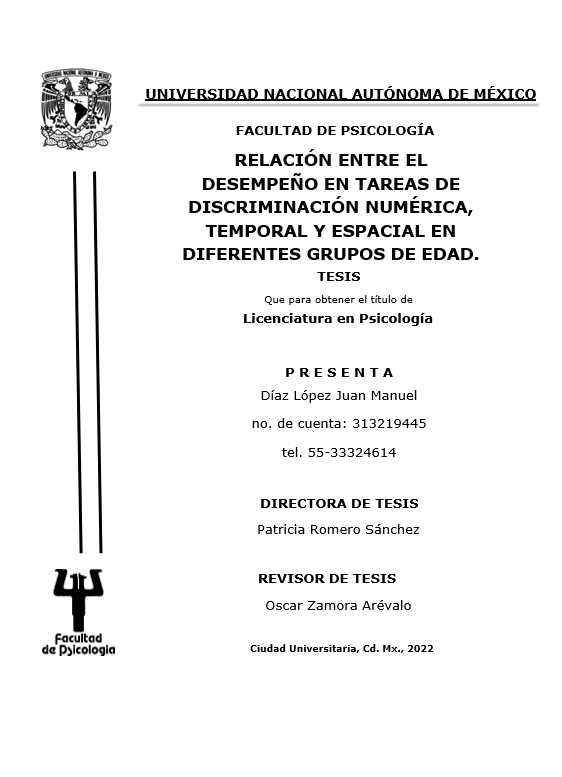
\includegraphics[width=\textwidth,height=0.75\textheight]{Anexos/Car_tit.png}

\href{https://tesiunam.dgb.unam.mx/F/2MNVUNLIDPT5Q7V34YD9J46DL8Y6R9P1SQU2KN9KVMCLKK7PN6-14675?func=find-b\&local_base=TES01\&request=Relaci\%C3\%B3n+entre+el+desempe\%C3\%B1o+en+tareas+de+discriminaci\%C3\%B3n+num\%C3\%A9rica\%2C+temporal+y+espacial+en+diferentes+grupos+de+edad\&find_code=WRD\&adjacent=N\&filter_code_2=WYR\&filter_request_2=\&filter_code_3=WYR\&filter_request_3=}{\textbf{LINK}}

\newpage

\hypertarget{formaciuxf3n-complementaruxeda}{%
\subsection{\texorpdfstring{\emph{Formación
complementaría}}{Formación complementaría}}\label{formaciuxf3n-complementaruxeda}}

\includegraphics[width=\textwidth,height=0.75\textheight]{Anexos/Const_4.png}


\includegraphics[width=\textwidth,height=0.75\textheight]{Anexos/2019-1_28_02.png}

\includegraphics[width=\textwidth,height=0.75\textheight]{Anexos/Const_3.png}


\includegraphics[width=\textwidth,height=0.75\textheight]{Anexos/2019-1_34_08.png}


\includegraphics[width=\textwidth,height=0.75\textheight]{Anexos/Diapositiva22.png}
\newpage

\hypertarget{ponencias-1}{%
\subsection{\texorpdfstring{\emph{Ponencias}}{Ponencias}}\label{ponencias-1}}

\includegraphics[width=\textwidth,height=0.75\textheight]{Anexos/Const_2.png}

\includegraphics[width=\textwidth,height=0.75\textheight]{Anexos/Const_1.png}


\includegraphics[width=\textwidth,height=0.75\textheight]{Anexos/Diapositiva6.png}


\label{LastPage}~
\end{document}
